\documentclass{standalone}
 
\usepackage{pgfplots}
% https://latexdraw.com/plot-a-function-and-data-in-latex/
\pgfplotsset{compat = newest}
 
\begin{document}
 
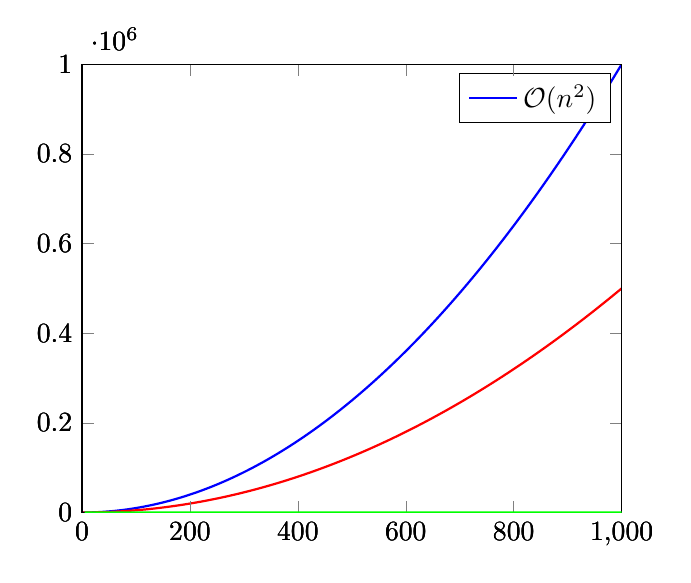
\begin{tikzpicture}
    \begin{axis}[
        xmin = 0, xmax = 1000,
        ymin = 0, ymax = 1000000]
        \addplot[
            domain = 0:1000,
            samples = 200,
            smooth,
            thick,
            blue,
        ]
        {x^2};
        \addlegendentry{$\mathcal{O}(n^2)$}
    \end{axis}
    \begin{axis}[
        xmin = 0, xmax = 1000,
        ymin = 0, ymax = 1000000]
        \addplot[
            domain = 0:1000,
            samples = 200,
            smooth,
            thick,
            red,
        ] %{exp(-x/10)*( cos(deg(x)) + sin(deg(x))/10 )};
        {(x^2)/2};
        

    \end{axis}
    \begin{axis}[
        xmin = 0, xmax = 1000,
        ymin = 0, ymax = 1000000]
        \addplot[
            domain = 0:1000,
            samples = 200,
            smooth,
            thick,
            green,
      ]
        {(x(log2(x)))};
    \end{axis}
\end{tikzpicture}
 
\end{document}